\textbf{1.\ (Filming a movie).}
A producer (Polly), an operator (Oliver) and a composer (Chris) are filming a
movie. The movie yields \(\$10000\) profit. Oliver himself can earn \(\$2000\)
by filming a wedding, Chris himself can earn \(\$3000\) by selling the music,
Polly herself can earn only \(\$1000\) by event management. Oliver and Chris
can earn \(\$6000\) by creating a music film for a wedding. Oliver and Polly
can earn \(\$4000\) by organizing the whole wedding. Polly and Chris can earn
\(\$4500\) by organizing a party.

\begin{enumerate}
    \item[(a)] Formalize the situation as a coalitional game. Is it superadditive?
    Supermodular?
    \item[(b)] Find the core and draw it on the plane (Polly payoff, Chris payoff).
    \item[(c)] Find the Shapley value. Does it lie inside the core?
\end{enumerate}

\textbf{Solution.}

Let
\[
N=\{P,O,C\},
\]
where \(P\) is Polly, \(O\) is Oliver, and \(C\) is Chris.

The payoff function is
\[
v(\varnothing)=0,
\]
\[
v(P)=1000,\qquad v(O)=2000,\qquad v(C)=3000,
\]
\[
v(PO)=4000,\qquad v(PC)=4500,\qquad v(OC)=6000,
\]
\[
v(POC)=10000
\]

The game is superadditive, since every coalition gives at least as much
as separate coalitions. Showing this:

\[
v(PO)=4000\ge v(P)+v(O)=1000+2000=3000,
\]
\[
v(PC)=4500\ge v(P)+v(C)=1000+3000=4000,
\]
\[
v(OC)=6000\ge v(O)+v(C)=2000+3000=5000,
\]
\[
v(POC)=10000\ge v(P)+v(OC)=1000+6000=7000,
\]
\[
v(POC)=10000\ge v(O)+v(PC)=2000+4500=6500,
\]
\[
v(POC)=10000\ge v(C)+v(PO)=3000+4000=7000
\]


Hence the game is superadditive.


Show supermodularity:
\[
v(POC)+v(P)\ge v(PO)+v(PC),
\]
because
\[
10000+1000=11000\ge 4000+4500=8500
\]
Similarly,
\[
v(POC)+v(O)\ge v(PO)+v(OC),
\]
because
\[
10000+2000=12000\ge 4000+6000=10000
\]
And
\[
v(POC)+v(C)\ge v(PC)+v(OC),
\]
because
\[
10000+3000=13000\ge 4500+6000=10500
\]
So, the game is supermodular.


\medskip
The core consists of allocations
\[
x=(x_P,x_O,x_C)
\]
such that
\[
x_P+x_O+x_C=10000,
\]
and
\[
x_P\ge1000,\qquad x_O\ge2000,\qquad x_C\ge3000,
\]
\[
x_P+x_O\ge4000,
\]
\[
x_P+x_C\ge4500,
\]
\[
x_O+x_C\ge6000
\]

To draw the core we use
\[
x_O=10000-x_P-x_C
\]

Then the constraints become
\[
1000\le x_P\le4000,
\]
\[
3000\le x_C\le6000,
\]
\[
4500\le x_P+x_C\le8000
\]

Hence the core is a hexagon with vertices
\[
(1000,3500),
\]
\[
(1500,3000),
\]
\[
(4000,3000),
\]
\[
(4000,4000),
\]
\[
(2000,6000),
\]
\[
(1000,6000)
\]

\begin{center}
    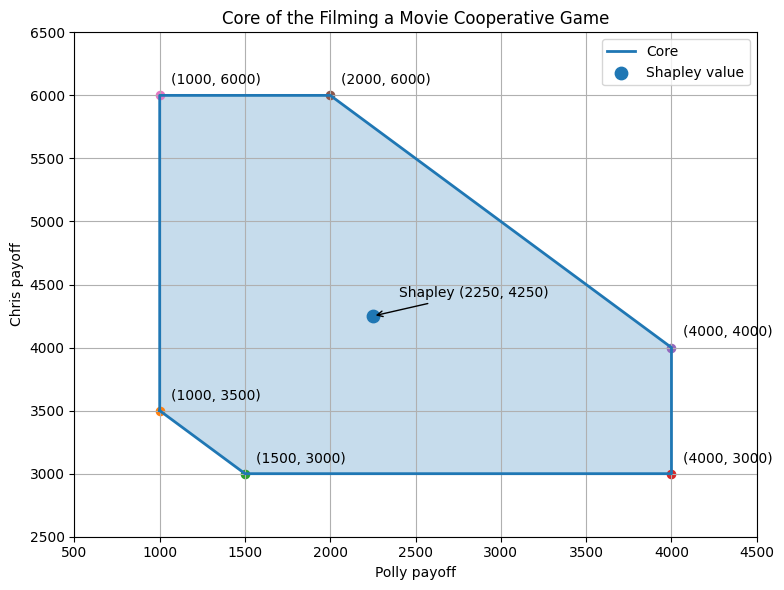
\includegraphics[width=1\textwidth]{problem3_1.png}
\end{center}

Now compute the Shapley value:

\[
\operatorname{sv}_P=\frac{1000+1000+2000+4000+1500+4000}{6}=2250,
\]
\[
\operatorname{sv}_O=\frac{3000+5500+2000+2000+5500+3000}{6}=3500,
\]
\[
\operatorname{sv}_C=\frac{6000+3500+6000+4000+3000+3000}{6}=4250
\]

\[
\begin{array}{c|ccc}
\text{Order} & P & O & C\\
\hline
POC & 1000 & 3000 & 6000\\
PCO & 1000 & 5500 & 3500\\
OPC & 2000 & 2000 & 6000\\
OCP & 4000 & 2000 & 4000\\
CPO & 1500 & 5500 & 3000\\
COP & 4000 & 3000 & 3000 \\
Shapley\ value & 2250 & 3500 & 4250
\end{array}
\]


Hence
\[
\operatorname{sv}(P,O,C)=(2250,3500,4250).
\]

Check whether it lies in the core:
\[
2250+3500+4250=10000,
\]
\[
2250\ge1000,\qquad 3500\ge2000,\qquad 4250\ge3000,
\]
\[
2250+3500=5750\ge4000,
\]
\[
2250+4250=6500\ge4500,
\]
\[
3500+4250=7750\ge6000
\]

Thus all core constraints are satisfied, so
\[
\operatorname{sv}(P,O,C)=(2250,3500,4250)\in \operatorname{Core}(v)
\]

Therefore,
\[
\text{the game is superadditive and supermodular,}
\]
and
\[
\text{the Shapley value lies inside the core}
\]
